\clearpage
\section{基于PauTa准则和Kalman滤波的去误差模型}
\subsection{模型的建立}
\subsubsection{PauTa准则}
PauTa\index{PauTa}准则,又称\(3\sigma\)准则。即有约99.7\%的概率相信服从正态分布的随机变量不会取与均值偏离3倍方差的区间外的值。
\begin{figure}[htbp]
	\centering
	\caption{PauTa准则}
	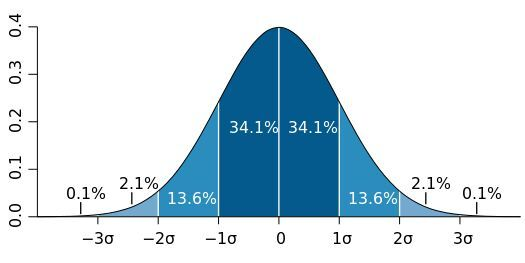
\includegraphics[width=8cm]{PauTa.jpg}
\end{figure}
\par 考虑到船舶实际加速度有限,对船舶加速度也进行了粗度误差的鉴别。根据PauTa准则,时空位置信息数据不含粗大误差,而信号特征信息数据经过剔除后每组指标的数值种类极少,有的如L1\_1甚至只有一种,故假设信号特征信息数据是信号源的唯一标识。所以最终每组信号特征信息数据指标为该组该指标的众数。推测可能是因为仪表读数在一开始有抖动现象,而测量人员在读数未趋于稳定之前记录读数导致。
\subsubsection{Kalman滤波}
\begin{figure}[htbp]
	\centering
	\caption{船舶所在海域}
	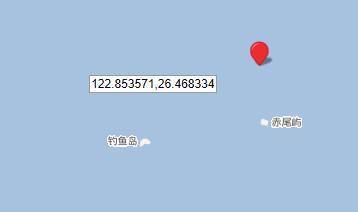
\includegraphics[width=8cm]{map.png}
\end{figure}
\par 一般船舶的航程事先确定,分为从起点码头离开时逐渐加速、途中保持尽可能的匀速直线运动,除非紧急避让障碍物时改变速率或转向以及按一开始的航程转向、抵达终点码头前逐渐减速3个阶段。题一未给出船舶航行的具体信息,但根据地图定位显示附件一船舶所在地区并无码头,应该是处于第二阶段。且船舶航程路线上未发现大的礁石,海域宽阔也无需转向,故假设理想情况船舶做匀速直线运动。
\\\indent 利用Kalman滤波对随机误差进行减小。综合测量和推测的结果得到一个更精准的估计。
\begin{description}
	\item[测量]理想情况下信号源做直线运动,利用最小二乘法求出最小二乘线作为理想运动轨迹,将每个数据离最小二乘线的距离视为误差,该误差服从以\(\bm{0}\)为均值的正态分布,该正态分布的方差就是测量的方差。
	\begin{align}
		\bm{e}	&	\sim\mathcal{N}(\bm{0},\bm{\Sigma})		\\
		\bm{e}	&	=\bm{x}-\bm{x}_0						\\
		\bm{x}	&	\sim\mathcal{N}(\bm{\mu},\bm{\Sigma})	\\
		\bm{\mu}	&	=\bm{x}_0
	\end{align}
	\par\(\bm{x}\)是表征通过测量确定坐标真实值概率分布的随机变量,\(\bm{x}_0\)是坐标测量值,\(\bm{e}\)是误差。
	\begin{figure}[htbp]
		\centering
		\begin{minipage}[htbp]{7.5cm}
			\centering
			\caption{原始数据}
			\includegraphics[width=7.5cm]{origin.eps}
		\end{minipage}
		\begin{minipage}[htbp]{7.5cm}
			\centering
			\caption{原始数据及其最小二乘线}
			\includegraphics[width=7.5cm]{LSQ.eps}
		\end{minipage}
	\end{figure}
	\item[推测]理想情况下信号源做匀速运动。求出每组所有相邻测量数据的平均速度,用平均速度代替瞬时速度。由于噪声服从正态分布假设坐标真实速度也服从正态分布,求出均值、方差。利用匀速直线运动的函数求出相邻2个数据的经纬度坐标的关系。代入第1个数据推测出第2个数据。
	\begin{align}
		\bm{v}		&	\sim\mathcal{N}(\bm{\mu'_v},\bm{\Sigma'_v})	\\
		\bm{x'}_0		&	\sim\mathcal{N}(\bm{\mu'}_0,\bm{\Sigma'}_0)	\\
		\bm{x'}		&	=\bm{x'}_0+\bm{v}\Delta t					\\
		\bm{x'}		&	\sim\mathcal{N}(\bm{\mu'},\bm{\Sigma'})		\\
		\bm{\mu'}		&	=\bm{\mu'}_0+\Delta t\bm{\mu'_v}				\\
		\bm{\Sigma'}	&	=\bm{\Sigma'}_0+\Delta t^2\bm{\Sigma'}_0
	\end{align}
	\par\(\Delta t\)是与上次测量间隔的时间,\(\bm{x}\bm{'}\)是表征通过推测确定坐标真实值概率分布的随机变量,\(\bm{v}\)是表征通过测量确定速度真实值概率分布的随机变量,\(\bm{x}\bm{'}_0\)是上次表征通过综合确定坐标真实值概率分布的随机变量,第一轮迭代时用上次的坐标测量值代替。
	\item[综合]综合测量和推测的结果以减小误差。
	\begin{align}
		&	\bm{x}\bm{''}\sim\mathcal{N}(\bm{\mu}\bm{''},\bm{\Sigma}\bm{''})												\\
		&	\mathcal{N}(\bm{\mu''},\bm{\Sigma''})=\mathcal{N}(\bm{\mu},\bm{\Sigma})\cdot\mathcal{N}(\bm{\mu'},\bm{\Sigma'})		\\
		&
		\begin{cases}
			\bm{\mu''}=\bm{\mu}+\bm{K}(\bm{\mu'}-\bm{\mu})	\\
			\bm{\Sigma''}=\bm{\Sigma}-\bm{K}\bm{\Sigma'}		\\
			\bm{K}=\bm{\Sigma}(\bm{\Sigma}+\bm{\Sigma'})^{-1}
		\end{cases}
	\end{align}
	\par\(\bm{K}\)被称为Kalman增益。\(\bm{x}\bm{''}\)是表征通过综合确定的坐标真实值概率分布的随机变量。
	\begin{figure}[htbp]
		\centering
		\begin{minipage}[htbp]{7.5cm}
			\centering
			\caption{俯视图}
			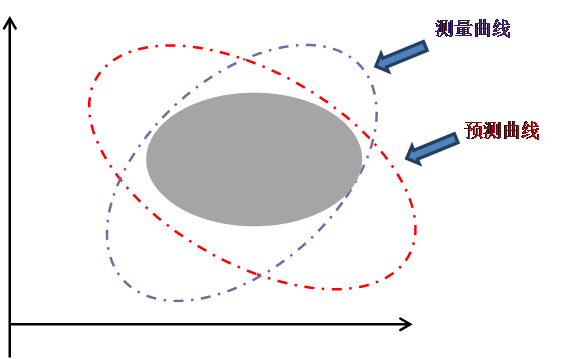
\includegraphics[width=6cm]{vertical.png}
		\end{minipage}
		\begin{minipage}[htbp]{7.5cm}
			\centering
			\caption{正视图}
			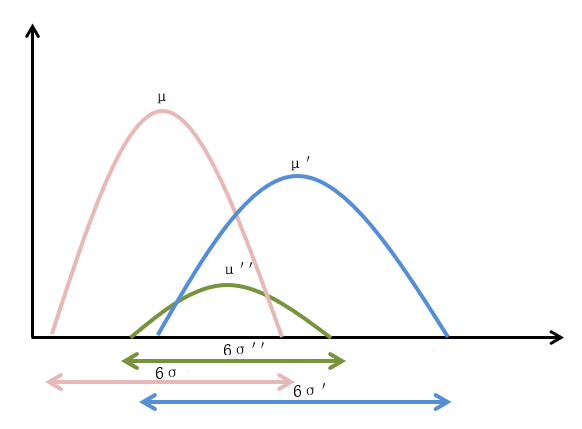
\includegraphics[width=6cm]{front.png}
		\end{minipage}
	\end{figure}
	\item[迭代]将\(\bm{x}\bm{''}\)作为下一轮迭代的\(\bm{x}\bm{'}_0\),重复以上过程不断迭代直至结束。
\end{description}
\subsection{模型的求解}
\begin{figure}[htbp]
	\centering
	\begin{minipage}[htbp]{7.5cm}
		\centering
		\caption{Kalman滤波后的数据及其最小二乘线}
		\includegraphics[width=7.5cm]{Kalman.eps}
	\end{minipage}
	\begin{minipage}[htbp]{7.5cm}
		\centering
		\caption{最小二乘线参数}
		\begin{tabular}{ccc}
			\toprule
			船舶编号	&	斜率			&	截距/经纬度		\\
			\midrule
			241		&	1.127344668	&	-114.027			\\
			379		&	1.121178211	&	-113.266			\\
			524		&	1.142658152	&	-115.944			\\
			658		&	2.137685441	&	-235.931			\\
			\bottomrule
		\end{tabular}
	\end{minipage}
\end{figure}
\par 根据PauTa准则数据的确信区间长度为6倍的标准差,故可用方差衡量误差导致的不确定度。
\begin{table}[htbp]
	\centering
	\caption{误差}
	\begin{tabular}{cc}
		\toprule
		\(|\bm{\Sigma}|\)	&	\(|\bm{\Sigma}\bm{'}|\)	\\
		\midrule
		6.01E-06			&	6.01E-06				\\
		9.75E-12			&	1.27E-28				\\
		5.11E-05			&	2.87E-05				\\
		9.18E-12			&	7.72E-29				\\
		\bottomrule
	\end{tabular}
\end{table}
\par\(\bm{\Sigma}\bm{'}\)是通过测量确定坐标真实值概率分布的随机变量\(\bm{x}\bm{'}\)的方差。单位都是1经纬度对应的长度的平方。可以看到误差在滤波后比滤波前显著减小。
\subsection{模型的检验}
\subsubsection{重测信度法}
由于缺乏多组数据对比,因此我们选用信度分析来检验结果一致性,以此判断模型的可靠性。通过重测信度法,对同一组数据进行多次相同的误差处理,分析最后数据均值与方差的一致程度。
\begin{table}[htbp]
	\centering
	\caption{重测信度法}
	\begin{tabular}{|c|c|c|c|c|}
		\hline
		\diagbox{滤波次数}{时空位置信息\\修正值/经纬度}{船舶编号}	&	241	&	379	&	524	&	658	\\\hline
		1	&	0.00016458	&	7.04E-07	&	0.002433	&	7.43E-06		\\\hline
		2	&	0.00016388	&	7.04E-07	&	0.002079	&	7.43E-06		\\\hline
		3	&	0.00016388	&	7.04E-07	&	0.001991	&	7.43E-06		\\\hline
		4	&	0.00016388	&	7.04E-07	&	0.001966	&	7.43E-06		\\\hline
		5	&	0.00016388	&	7.04E-07	&	0.001957	&	7.43E-06		\\\hline
		6	&	0.00016388	&	7.04E-07	&	0.001955	&	7.43E-06		\\\hline
		7	&	0.00016388	&	7.04E-07	&	0.001954	&	7.43E-06		\\\hline
		8	&	0.00016388	&	7.04E-07	&	0.001954	&	7.43E-06		\\\hline
		9	&	0.00016388	&	7.04E-07	&	0.001954	&	7.43E-06		\\\hline
		10	&	0.00016388	&	7.04E-07	&	0.001954	&	7.43E-06		\\\hline
		11	&	0.00016388	&	7.04E-07	&	0.001954	&	7.43E-06		\\\hline
		12	&	0.00016388	&	7.04E-07	&	0.001954	&	7.43E-06		\\\hline
		13	&	0			&	7.04E-07	&	0.001954	&	7.43E-06		\\\hline
		14	&	0			&	0		&	0.001954	&	0			\\\hline
		15	&	0			&	0		&	0.001954	&	0			\\\hline
		16	&	0			&	0		&	0.001954	&	0			\\\hline
	\end{tabular}
\end{table}
\par 时空位置信息最大修正值为滤波后与原始数据的最大差值。经过多次Kalman滤波后数据结果趋于稳定。

